%========================================================================================
% TU Dortmund, Informatik Lehrstuhl VII
%========================================================================================

\chapter{Anwendung des Spring-Embedders auf den modellierten Graphen}
\label{Kapitel 4}
%

Der in Kapitel 3 vorgestellte Algorithmus wird nun so erweitert und angepasst, dass er für den gegebenen Graphen und unser Problem passend ist. Das Ziel wird es sein, den aus Kapitel 2 gewonnen Graphen mithilfe des Algorithmus zu einer MetroMap ähnlichen Darstellung zu führen. Die besonders leichte Erweiterbarkeit und Modifizierbarkeit des Algorithmus erlauben dies und ist auch der Grund, weshalb dieser Algorithmus als Basis zur Lösung des Problems verwendet wurde. \\

\section{Vergleich des vom Algorithmus erhaltenen Layout mit dem einer MetroMap}
\label{Kapitel_4_-_Unterkapitel_2}

Das Erstellen dieses Layouts im Vergleich zur herkömmlichen MetroMap unterscheidet sich vor allem durch:

\begin{itemize}
	\item eine deutlich striktere Beibehaltung der topologischen und geographischen Eigenschaft des Graphen
	\item das Verteilen der Knoten auf die komplette Oberfläche soll nicht stattfinden
	\item es existieren Knoten, die sich nicht bewegen lassen
	\item durch das modellieren der Leiterseile existiert eine bestimmte Struktur innerhalb des Graphen, die noch immer sichtbar bleiben soll
	\item nichts außerhalb des Platzierens von Knoten und Kanten wird angewendet, das sind vor allem, bei einer MetroMap, das Erstellen von Labels und die Färbung von Kanten.
\end{itemize} 

Der vorgestellte Algorithmus in Kapitel 3 wandelt einen Graphen ebenso nicht in eine perfekte MetroMap um. Orthogonalität wird komplett ignoriert. Durch das zufällige Platzieren der Knoten, wird jegliche Topologie des Graphen entfernt und alle anderen ausmachenden Komponenten einer MetroMap werden nicht erstellt. Ausschließlich das Platzieren der Knoten und Kanten sind beim Erstellen des neuen Layouts von Bedeutung, dh. es wird bei der Platzierung auch nicht auf mögliche Positionen der Labels geachtet. Das Ziel ist es demnach nun den Algorithmus den neuen Ansprüchen anzupassen und ein ansprechendes Layout des Ausschnittes des Höchstspannungsnetzes zu erstellen. Dieser Ausschnitt  kann anschließend beliebig erweitert werden oder das komplette Höchstspannungsnetz umfassen.  


\section{Nachteile des Spring-Embedders auf der Anwendung des Graphen}
\label{Kapitel_4_-_Unterkapitel_2}

\begin{figure}[t]
	\centering
	{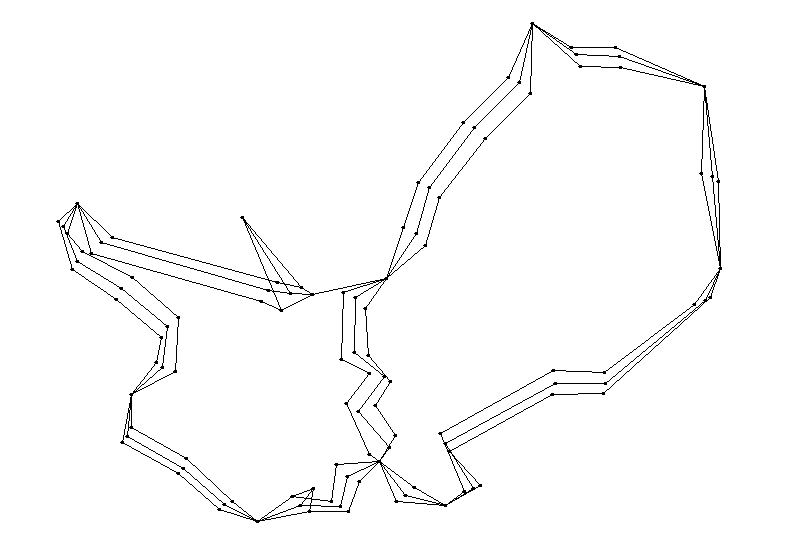
\includegraphics[scale=0.8]{bilder/graph10iterationenreingold}\label{fig_dortmundmap}
	}\\
	\caption[Dortmunder MetroMap]{Dortmunder MetroMap [http://www.urbanrail.net/eu/de/do/dortmund-map.png]}
	\label{fig_dortmundmap}
\end{figure}
\begin{figure}[t]
	\centering
	{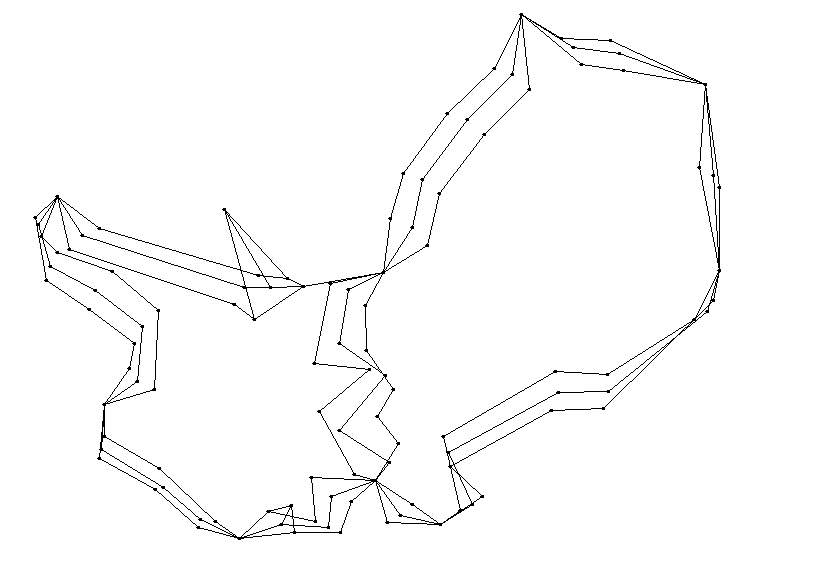
\includegraphics[scale=0.8]{bilder/graph25iterationenreingold}\label{fig_dortmundmap}
	}\\
	\caption[Dortmunder MetroMap]{Dortmunder MetroMap [http://www.urbanrail.net/eu/de/do/dortmund-map.png]}
	\label{fig_dortmundmap}
\end{figure}
\begin{figure}[t]
	\centering
	{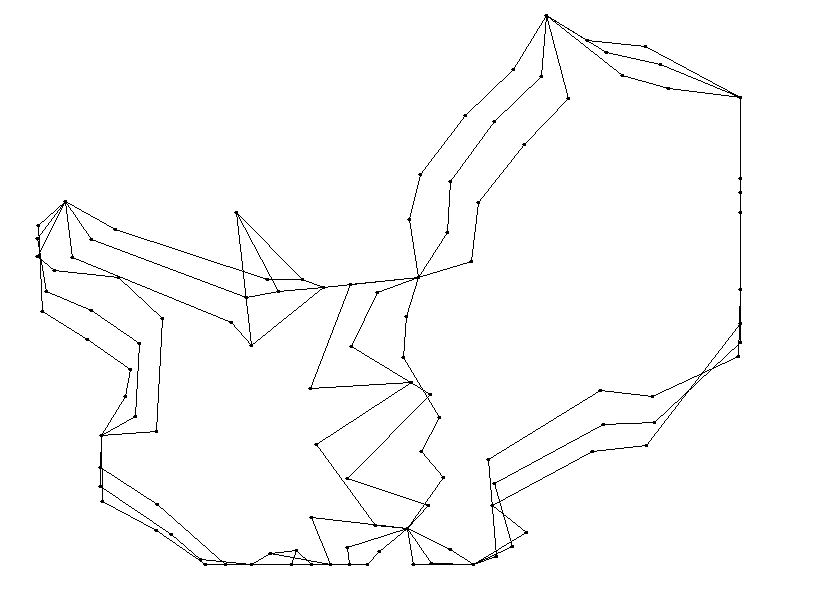
\includegraphics[scale=0.8]{bilder/graph50iterationenreingold}\label{fig_dortmundmap}
	}\\
	\caption[Dortmunder MetroMap]{Dortmunder MetroMap [http://www.urbanrail.net/eu/de/do/dortmund-map.png]}
	\label{fig_dortmundmap}
\end{figure}
Im Folgenden wird der Algorithmus unmodifiziert auf den Graphen angewendet um deutlich zu machen, wo die grundsätzlichen Probleme dieses Algorithmus liegen und was verbessert werden muss. Dazu wird dieser mit einer verschiedenen Anzahl an Iterationen auf den Graphen angewendet und anschließend ausgewertet. Existierten keine Bewegungseinschränkungen für die Knoten und würde der Algorithmus so auf den Graphen angewendet werden, würden viele unerwünschte Nebeneffekte eintreten, die den Graphen noch unästhetischer machen. In den Abbildung 4.1/2/3 wird der resultierende Graph dargestellt nach jeweils 10, 25 und 50 Iterationen.\\

Nach 10 Iterationen des Algorithmus wird eine deutliche Verbesserung der Abstände der Knoten sichtbar. Das resultiert aus der abstoßenden Kraft der Knoten zueinander. Jedoch treten bei 10 Iterationen schon große Probleme mit der Überschneidung von Kanten auf, was eine nicht planare Darstellung des Graphen zur Folge hat. Dies sollte jedoch unter allen Umständen vermieden werden, denn wie es auf der Abbildung 4.1 schon leicht zu sehen ist, wird durch das Überschneiden von Knoten der Graph sehr unübersichtlich und es wird schwer zu sagen, zu welcher Kante welcher Knoten gehört. Da die vergrößerten Abstände der Knoten auf den langen Verbindungen zu einer deutlichen Verbesserung der Ästhetik führen, sieht der resultierende Graph nach 10 Iterationen, trotz der leichten Überschneidung von Kanten, schon deutlich übersichtlicher aus. \\

Nach weiteren Iterationen des Algorithmus wird die Darstellung zunehmend schlechter und es kommt zu etlichen Überschneidungen der Kanten. Die Knoten stoßen sich weiter ab und sie fangen an sich an die Grenzen der Oberfläche zu bewegen, welches auf der Abbildung 4.2 nach 25 Iterationen am linken, rechten und unteren Rand gut zu sehen ist. Die Knoten fangen an sich dort zu sammeln und trotz ihrer abstoßenden Kraft zueinander wird das Sammeln zunehmend schlimmer. Der ursprüngliche Graph, welcher aus dem Höchstspannungsnetz modelliert wurde, ist noch immer wiederzuerkennen. Die beiden markanten großen Flächen innerhalb des Graphen, welche der ursprüngliche Graph auch besaß, sind noch deutlich zu erkennen. Der Zweck des Algorithmus die Knoten gleichmäßig zu verteilen mit einer optimalen Distanz zu einander wird langsam deutlich durch die größeren Abstände der Knoten. \\

Nach 50 Iterationen, welches auf Abbildug 4.3 zu sehen ist, sind fast alle Knoten bereits deutlich von ihrer Startpositionen bewegt worden. Ursprüngliche Muster, Merkmale oder die Wiedererkennbarkeit dieser Zeichnung im Vergleich des Graphen vor Anwendung des Algorithmus, wird immer schwerer. Die äußeren Grenzen sind sehr deutlich am Rande der Oberfläche zu sehen. Die Knoten sammeln sich dort, da sie sich nicht weiter nach außen entfernen können. Die anderen Knoten fangen an sich in den beiden offenen Flächen des Graphen zu verteilen und zu Positionieren. Es scheint als wäre die Oberfläche nicht groß genug für den Algorithmus mit der gegebenen Anzahl an Knoten, doch auch eine deutliche Verringerung der Knoten führt zum selben Ergebnis, da die optimale Distanz zwischen zwei Knoten noch deutlich zu groß ist. Die Knoten versuchen sich ausnahmslos auf der Oberfläche mit perfekten Abständen zu einander zu verteilen. Dieser Vorgang ist jedoch nicht gewollt, nicht bei dem Layout unseres Graphen noch bei einer grundsätzlichen MetroMap. Es gibt auch sehr viele Ausreißer, die ein lokales Minima nicht mehr überwinden können. Das bedeutet, der Algorithmus wird niemals, eine erst schlechtere Positionierung wählen um anschließend eine bessere zu bekommen. Er wird stets versuchen von Iteration nach Iteration eine bessere Positionierung anhand der Kräfte zu erhalten, auch wenn dies zur Folge hat, dass die Knoten sich möglicherweise nicht optimal Positionieren. \\


\section{Anpassung des Spring-Embedders zur Anwendung auf das modellierte Höchstspannungsnetz}
\label{Kapitel_4_-_Unterkapitel_3}

\begin{figure}[t]
	\centering
	{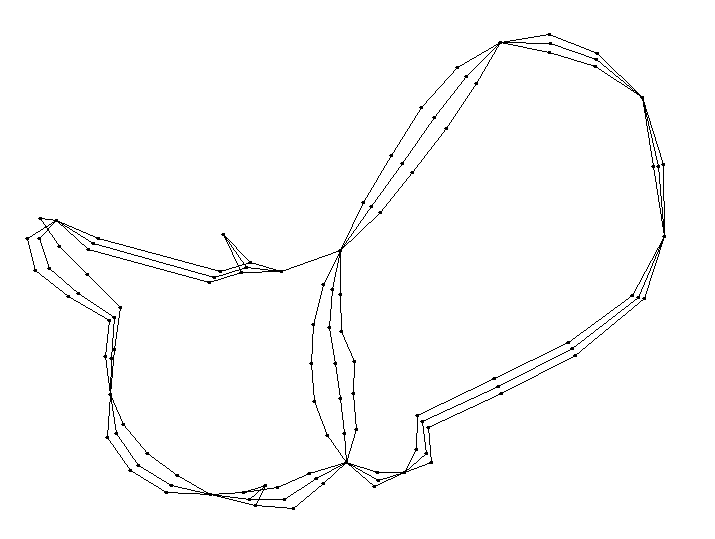
\includegraphics[scale=0.8]{bilder/graph25iterationenreingoldmodified1}\label{fig_dortmundmap}
	}\\
	\caption[Dortmunder MetroMap]{Dortmunder MetroMap [http://www.urbanrail.net/eu/de/do/dortmund-map.png]}
	\label{fig_dortmundmap}
\end{figure}
\begin{figure}[t]
	\centering
	{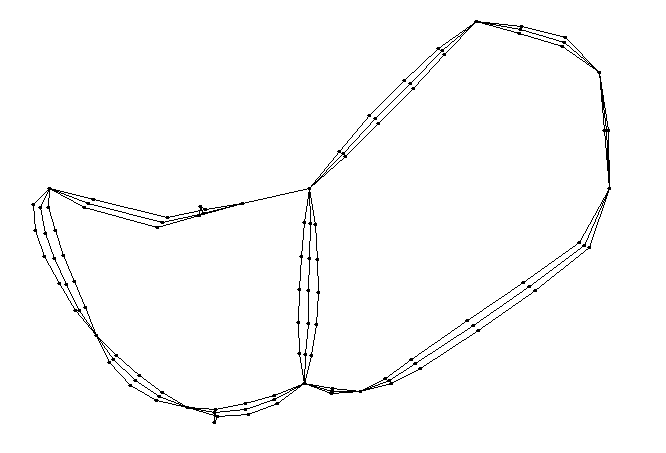
\includegraphics[scale=0.8]{bilder/graph50iterationenreingoldmodified1}\label{fig_dortmundmap}
	}\\
	\caption[Dortmunder MetroMap]{Dortmunder MetroMap [http://www.urbanrail.net/eu/de/do/dortmund-map.png]}
	\label{fig_dortmundmap}
\end{figure}

Zum Anwenden auf das Höchstspannungsnetz war der Algorithmus in seiner ursprünglichen Form nicht geeignet, besonders nicht mit der zur Hinzunahme der erweiterten Regeln die zum Erstellen des Layouts gelten. Nun geht es demnach darum, den Algorithmus so anzupassen, dass er ein passendes Layout des Graphen liefert, der die Anforderung besser erfüllt. Der Algorithmus kann demnach auf viele verschiedene Arten erweitert oder verändert werden. \\

Eine bereits deutliche Besserung des Layouts führt eine Veränderung der optimalen Distanz. Die Konstante $C$ bei der Berechnung der optimalen Distanz	$k = C\sqrt{A / |V|}$ sollte so gewählt werden, dass sie die optimale Distanz zwischen zwei benachbarten Knoten deutlich verringert, damit diese nicht mehr auf der kompletten Oberfläche verteilt werden und so schnell zum Rand der Zeichnung driften. Auf der Abbildung 4.4 ist der selbige Algorithmus wie bei Abbildung 4.2 zu sehen, ebenfalls mit 25 Iterationen, jedoch wurde die Konstante $C$ auf $1/8$ gesetzt, die optimale Distanz die der Algorithmus für benachbarte Knoten versucht zu erreichen, wurde demnach durch acht geteilt. Es gibt noch immer einige Ausreißer aber die Überschneidungen von Kanten hat sich reduziert und die Knoten scheinen geordneter zu liegen. Generell scheint die Zeichnung des Graphen nun symmetrischer aber die Leiterseile haben etwas an ihrer Parallelität verloren.\\


Die Konstante $C$ wurde in Abbildung 4.5 sogar auf 1/16 gesetzt mit 50 Iterationen und trug damit zur deutlichen Verbesserung der Ästhetik des Layout bei. Wird die optimale Distanz zu sehr verringert, so ist, wie auf der Abbildung zu sehen, eine deutliche Abschwächung der Einflussnahme der abstoßenden Kraft zu sehen. Das hat zur Folge, dass die Knoten sich zu nahe kommen, was daraus resultiert, dass die Distanz zweier benachbarten Knoten so klein ist, dass sie sich lieber weiter verringert, als dass sich Knoten abstoßen wollen. Ein positiver Effekt der daraus folgt ist, dass sich kein Knoten mehr am Rand der Oberfläche sammelt. Ebenfalls sehr deutlich wird der komplette Verlust der topologischen Eigenschaften der Verbindungen. Jegliches umgangenes Hindernis ist in der Zeichnung nicht mehr zu sehen. Die Knoten haben sich komplett von ihrem Ursprung entfernt, dass die kompletten Merkmale und Eigenarten verschwunden sind. Es muss darauf geachtet werden, dass diese noch zu Erkennen sind und die optimale Distanz zweier benachbarter Knoten nicht zu sehr verringert wird. \\

Es können demnach viele Probleme nur mit Anpassung der optimalen Distanz gelöst werden, doch es folgen daraus Probleme die den Verlust der Topologie und geographischen Merkmale zur Folge haben. Ebenfalls wird die Parallelität der Leiterseile, welche einen guten Überblick der Verbindung verschafft, durch die optimale Distanz verringert. \\

\begin{algorithm}[t]
	\centering
	\caption[Erweiterung des Spring-Algorithmus]{Erweiterung des Spring-Algorithmus} \label{algo_2}
	\begin{algorithmic}[1]
		\REQUIRE \begin{math} G:= (V,E) \end{math}
		\ENSURE \begin{math} G:= (V,E) \end{math}
		\FOR{\begin{math}i:=1 \leq iterations \end{math}}
		\STATE ..
		\newline
		\FOR{\begin{math}e_{v_{i},v_{j}} \in E\end{math}}
		\STATE $\Delta := p_{v_{i}} - p^{0}_{v_{i}};$
		\STATE $d_{v_{i}} := d_{v_{i}} - (\Delta / |\Delta|) \cdot f^{a}_{v_{i},p^{0}_{v_{i}}}(|\Delta|));$
		\ENDFOR
		\newline
		\STATE ..
		\ENDFOR
	\end{algorithmic}
\end{algorithm}

Durch das Verändern der wirkenden Kräfte, können wiederum Nachteile der Veränderung der optimalen Distanz ausgeglichen werden. Wie bereits angesprochen, verliert die abstoßende Kraft zwischen den Knoten ihre Relevanz im Vergleich zur optimalen Distanz, sofern diese zu gering wird. Es ist sehr leicht diese Kraft etwas zu modifizieren und höher zu setzen und damit wieder mehr Konturen in das Layout bekommen. Die Topologie wird mehr beachtet und dennoch sammeln sich die Knoten nicht mehr Rande der Oberfläche. Wird die abstoßende Kraft des Algorithmus um etwa 40\% erhöht. so gibt es jedoch weitaus mehr Ausreißer, die die eigentliche Struktur komplett verlassen und nach außen driften. \\
\begin{figure}[t]
\centering
{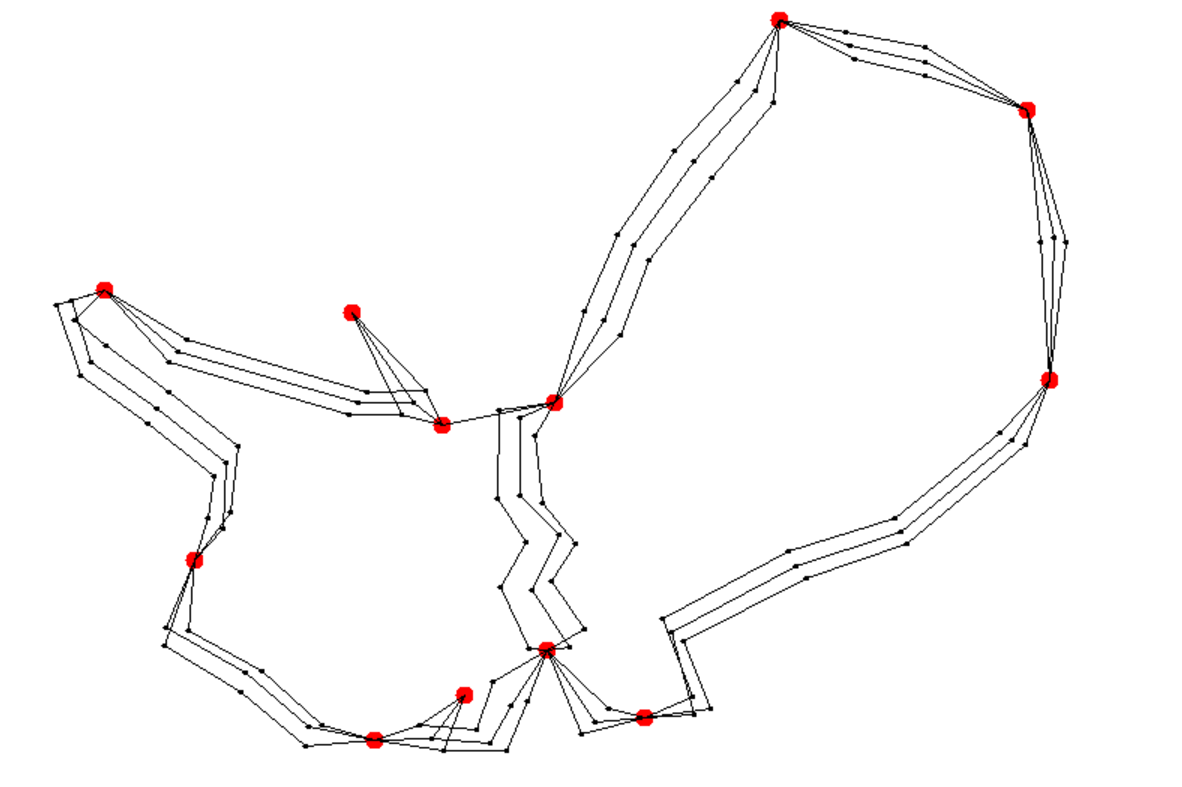
\includegraphics[scale=0.5]{bilder/graphfertig}\label{fig_dortmundmap}
}\\
\caption[Dortmunder MetroMap]{Dortmunder MetroMap [http://www.urbanrail.net/eu/de/do/dortmund-map.png]}
\label{fig_dortmundmap}
\end{figure}
Um das Problem der Ausreißer besser in den Griff zu bekommen und dennoch wieder mehr Topologie in dem Graphen zu bringen, ist es besser eine gänzlich neue Kraft der Abstoßenden und Anziehenden hinzuzufügen. Eine Kraft die nur sicherstellt, dass die Topologie des Graphen beibehalten wird. Das bedeutet die Knoten dürfen sich nicht zu weit von ihrer ursprünglichen Position entfernen. Die Kraft sollte stärker wirken, je weiter die Knoten von ihrer Startposition entfernt sind. Ähnlich der anziehenden Kraft zwischen zwei Knoten, die bereits vorhanden ist. Es müssen sich demnach alle Knoten ihre Startposition merken und stets mit ihrer momentanen Position vergleichen. Mithilfe dieser beiden Informationen, kann eine weitere anziehende Kraft hinzugefügt werden, welche mit diesen beiden Positionen arbeitet. Das Vorgehen dabei ist relativ simpel. Wird die anziehende Kraft so modifiziert, dass der zweite Knoten nicht mehr ein Knoten ist, sondern die ursprüngliche Position $p^{0}$ des ersten Knotens. So würde es nun eine anziehende Kraft von einem Knoten zu seiner Startposition geben. Diese Kraft muss natürlich auch jede Iteration auf jedem Knoten wirken und genau wie bei der ursprünglichen anziehenden Kraft, dem Vektor des Knotens, welcher die Richtung der Bewegung bestimmt hinzugefügt werden. Dem Algorithmus aus 3.1 wird demnach eine neue anziehende Kraft hinzugefügt, welche im Algorithmus 4.1 durch Zeile 3-6 veranschaulicht wird. Sie ist sehr ähnlich der anziehenden Kraft, nur dass der zweite Knoten durch die ursprüngliche Position $p^{0}$ ersetzt wird. \\
 


Es existieren nun jedoch wieder zu viele anziehende Kräfte, sodass die abstoßende Kraft in Relevanz zu schwach wirkt und die Knoten sich wieder näher zueinander hinziehen als sie sollten. Um das Problem der Ausreißer weitestgehend zu verhindern, wird die abstoßende Kraft nicht erhöht, sondern die beiden anziehenden Kräfte verringert. Experimentell hat sich bewährt, dass eine Schwächung der anziehenden Kraft zwischen benachbarten Knoten von etwa 20\% und eine Schwächung von 50\% der haltenden Kraft, die einen Knoten an ihre ursprüngliche Position hält, die schönsten Layouts bringt, die sich am besten dem Problem angepasst haben. \\

\begin{figure}[t]
	\centering
	\subfigure[deutlich vergrößerter Abstand zwischen den Knoten, der Verlauf wurde jedoch beibehalten]
	{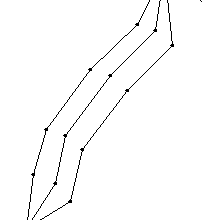
\includegraphics[scale=1.0]{bilder/abstandseile}\label{fig_planar1}
	}
	\hspace{1.0cm}%
	\subfigure[Der Graph mit den modellierten Leiterseilen]
	{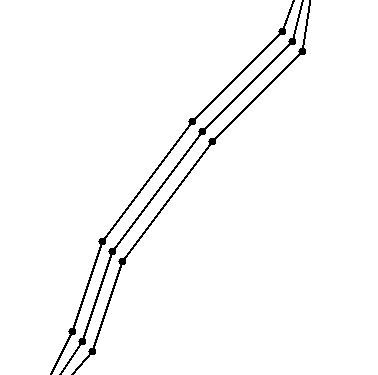
\includegraphics[scale=0.5]{bilder/knotenplacement}\label{fig_planar2}
	}
	\\
	\caption[Vergleich der Leiterseile]{Modellierung der Leiterseile}
	\label{fig_testbild2}
\end{figure}


Auf der Abbildung 4.6 ist das Endergebnis  der Arbeit zu sehen. Fast alle Knoten haben einen guten Abstand zueinander, welches auch in Abbildung 4.7 dargestellt wird.  Die Verbindungen sind noch sehr ähnlich ihrem ursprünglichen geographischen Verlauf. Es ist kein Problem zu erkennen, wo die umgangenen Hindernisse sich befanden. Drei Ausreißer sind noch zu sehen, welche sich jedoch nur sehr schwer entfernen lassen. Die Parallelität zwischen den Leiterseilen ist sehr gut zu sehen. Es ist nun möglich bei jeder Verbindung die Anzahl der Leiterseile direkt der Zeichnung zu entnehmen.

\section{Bildung nahezu paralleler Leiterseile mittels dem Spring-Embedder}
\label{Kapitel_4_-_Unterkapitel_4}

\begin{figure}[t]
	\centering
	\subfigure[Die roten Knoten repräsentieren unbewegliche Städte, zwischen ihnen verlaufen genau drei Leiterseile, die noch einen parallelen Verlauf aufweisen]
	{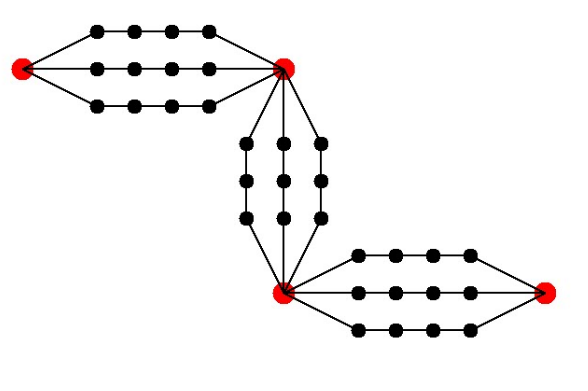
\includegraphics[scale=0.6]{bilder/bildungschlangen1}\label{fig_planar1}
	}
	\hspace{1.0cm}%
	\subfigure[Nach der Anwendung des Algorithmus auf den Graphen geht die parallele Struktur verloren]
	{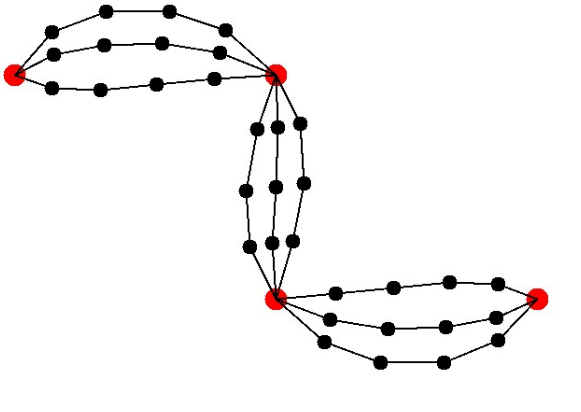
\includegraphics[scale=0.6]{bilder/bildungschlangen2}\label{fig_planar2}
	}
	\\
	\caption[Aus der parallelen Struktur des Graphen wird durch den Algorithmus eine kurvige]{Aus der parallelen Struktur des Graphen wird durch den Algorithmus eine kurvige}
	\label{fig_testbild2}
\end{figure}

\begin{figure}[t]
	\centering
	\subfigure[Die roten Knoten repräsentieren unbewegliche Städte, zwischen ihnen verlaufen genau drei Leiterseile, die noch einen parallelen Verlauf aufweisen]
	{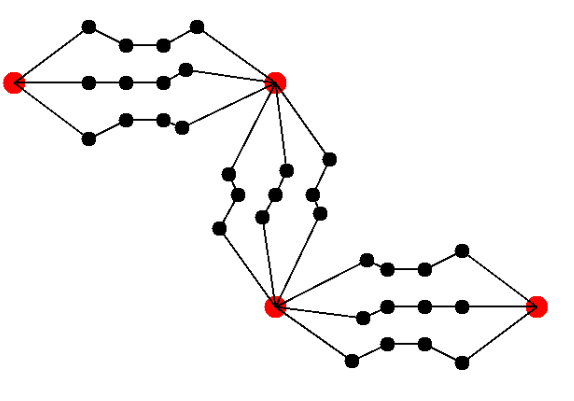
\includegraphics[scale=0.6]{bilder/bildungschlangen3}\label{fig_planar1}
	}
	\hspace{1.0cm}%
	\subfigure[Nach der Anwendung des Algorithmus auf den Graphen geht die parallele Struktur verloren]
	{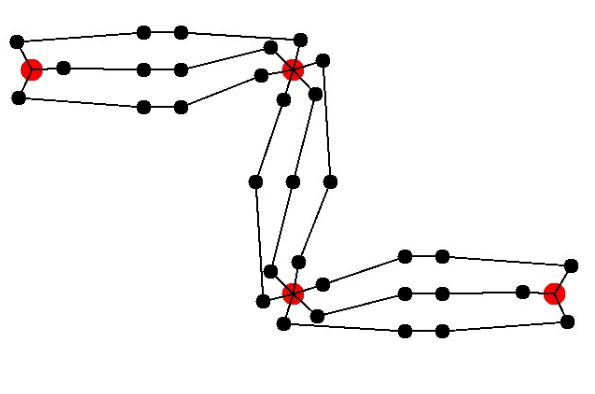
\includegraphics[scale=0.6]{bilder/bildungschlangen4}\label{fig_planar2}
	}
	\\
	\caption[Aus der parallelen Struktur des Graphen wird durch den Algorithmus eine kurvige]{Aus der parallelen Struktur des Graphen wird durch den Algorithmus eine kurvige}
	\label{fig_testbild2}
\end{figure}

\begin{figure}[t]
	\centering
	\subfigure[Die roten Knoten repräsentieren unbewegliche Städte, zwischen ihnen verlaufen genau drei Leiterseile, die noch einen parallelen Verlauf aufweisen]
	{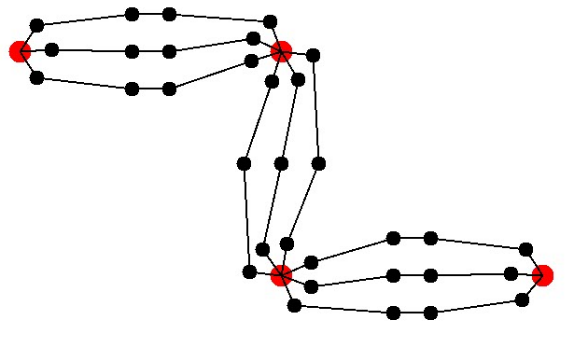
\includegraphics[scale=0.6]{bilder/bildungschlangen5}\label{fig_planar1}
	}
	\hspace{1.0cm}%
	\subfigure[Nach der Anwendung des Algorithmus auf den Graphen geht die parallele Struktur verloren]
	{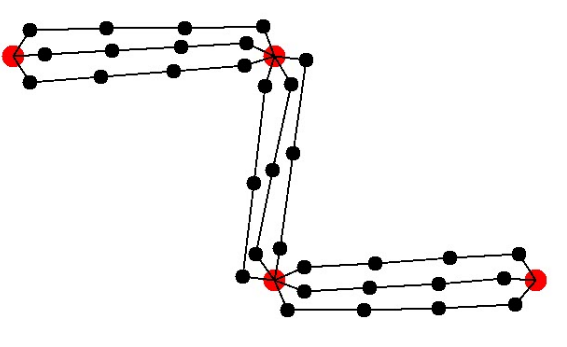
\includegraphics[scale=0.6]{bilder/bildungschlangen7}\label{fig_planar2}
	}
	\hspace{1.0cm}%
	\subfigure[Die roten Knoten repräsentieren unbewegliche Städte, zwischen ihnen verlaufen genau drei Leiterseile, die noch einen parallelen Verlauf aufweisen]
	{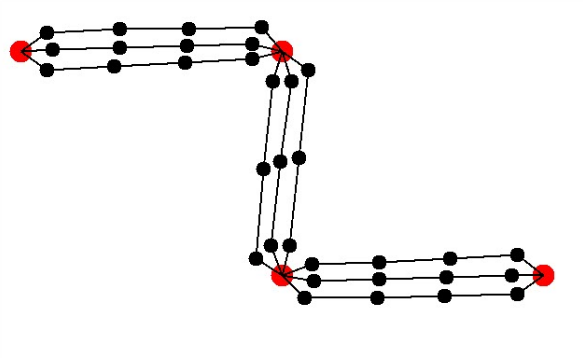
\includegraphics[scale=0.6]{bilder/bildungschlangen8}\label{fig_planar1}
	}
	\\
	\caption[Aus der parallelen Struktur des Graphen wird durch den Algorithmus eine kurvige]{Aus der parallelen Struktur des Graphen wird durch den Algorithmus eine kurvige}
	\label{fig_testbild2}
\end{figure}

Um eine noch bessere Sichtbarkeit der Parallelität zu schaffen, wurde eine weitere Kraft hinzugefügt. Diese Kraft verändert nicht nur die Parallelität der Leiterseile, sondern hat auch einen positiven Einfluss auf die Knoten, die in direkter Verbindung mit den größeren unbeweglichen Städten stehen. Das eigentliche Ziel war es die Bildung von Kurven in den Verbindungen zu verhindern. Durch die optimale Distanz bildet der Algorithmus eine rundliche Positionierung der Knoten um die unbeweglichen Städte. In der Abbildung 4.8 wird dieses Vorgehen anhand eines Beispielgraphen verdeutlicht. Die Städte und somit unbeweglichen Knoten sind rot. Die anderen Knoten haben eine kurvige Form in den Verbindungen. Dadurch wurde die Parallelität der Leiterseile aufgehoben. Ein Ziel war es jedoch, die Leiterseile so parallel wie möglich zu zeichnen, damit es leicht möglich ist zu sehen, in welcher Anzahl diese Auftreten und wie diese Verlaufen. Das folgende Verfahren verschiebt die Knoten so, dass keine kurvigen Kanten durch Anwendung des Algorithmus auftreten. \\

Es ist eine ziemliche Herausforderung, einem Algorithmus, der grundsätzlich eher kurvige Strukturen erzeugt dazu zu bringen parallel zu bleiben. Die Grundidee für das Folgende Vorgehen war es, die Städte, die direkt an einem Knoten liegen, sich anziehen zu lassen. Dadurch ist die bestmögliche Lösung, zur Platzierung der Knoten, eine indem die Knoten den geringsten Abstand zu einander haben und genau das ist der Fall, wenn sie sich direkt auf einer Gerade befinden. Ziehen sich diese jeweiligen Knoten an, so passiert es, dass sich die Knoten an den Städten zu nahe kommen, was eine unschönes Layout zur Folge hätte. \\

Der erste Schritt besteht darin, die Knoten, die in direkter Verbindung zu einem unbeweglichen Knoten stehen, sich abstoßen zu lassen. Diese Knoten sollen sich rundum an ihrem unbeweglichen Knoten verteilen. In der Abbildung 4.9(a) wird dargestellt wie sich die Knoten jeweils um den unbeweglichen Knoten verteilen und sich stark voneinander abstoßen. Damit sie sich jedoch nicht zu weit entfernen, wurde die optimale Distanz zwischen dem beweglichen und unbeweglichen Knoten sehr stark gesetzt, was zur Folge hat, dass sich diese auch wirklich um den Knoten verteilen und sich nicht immer weiter davon entfernen. Dies ist zu sehen in der Abbildung 4.9(b). Besonders gut zu sehen ist die perfekt symmetrische Verteilung der beweglichen Knoten um den unbeweglichen herum. Diese Knoten stoßen sich gegenseitig ab, werden aber stark durch den beweglichen angezogen, was diese Struktur zur Folge hat. Auf die anderen Knoten wird erst später ein justierende Kraft angewendet, deswegen liegen diese noch auf ihrer ursprünglichen Position. Durch diesen Ansatz müssen die noch unbewegten Knoten am Ende nur gut zwischen den zwei bis jetzt bewegten Knoten verteilt werden.\\


Da die Knoten nun sehr symmetrisch um die Städte positioniert wurden, müssen nun die Knoten gefunden werden, die sich direkt an einem unbeweglichen Knoten befinden und ihren direkten Partner am anderen Ende des Leiterseiles. Wurden diese beiden Knoten gefunden, die sich auf einem Leiterseil befinden und sich auch durch eine Kante in direkter Verbindung mit einem unbeweglichen Knoten stehen, so ist es möglich ihnen eine sehr leichte anziehende Kraft zu geben. Diese anziehende Kraft sorgt dafür, dass sich die Knoten nun nicht mehr nur um ihre Städte verteilen. Es wird die Struktur der Leiterseile wieder deutlicher. Dieser Vorgang wird in der Abbildung 4.10(a) gezeigt. Anstatt, dass sie sich nur noch um den Knoten verteilen, führt die leichte Einführung einer anziehenden Kraft nun dazu, dass sie wieder die Leiterseil ähnliche Form bekommen.\\

Die nicht bewegten Knoten in der Abbildung 4.10(a) werden nun auf die Verbindung ihrer Leiterseile gebracht und mit genug Abstand, damit sie sich gut verteilen. Dies führt zu der Abbildung 4.10(b), wo sich die bisher nicht bewegten Knoten nun zwischen dem Start- und Endknoten, welche den Start und das Ende des Leiterseiles modellieren, positionieren. Dies passiert nur durch die Einführung der anziehenden und abstoßenden Kraft, wie es bereits im Algorithmus 3.1 passiert ist. Hier ist bereits gut zu erkennen, dass die Leiterseile wieder sehr gerade verlaufen und keine Kurve bilden. \\

Im letzten Schritt wird versucht, die Leiterseile sich etwas paralleler ausrichten zu lassen, indem die optimale Distanz zwischen den Knoten verringert wurde, was zur Folge hat, dass sich die Knoten besser auf den Leiterseilen verteilen und sich generell etwas mehr zusammenziehen. Dieser Schritt ist in der Abbildung 4.10(c) zu sehen. Die Leiterseile dieses Graphen liegen nun fast komplett parallel zueinander und die anfänglich kurvige Form ist verschwunden. \\

\section{Einbettung der Knoten in Felder}
\label{Kapitel_4_-_Unterkapitel_4}

Es ist möglich, die Oberfläche in einzelne kleine Felder einzuteilen. In jedes dieser Felder passt anschließend genau ein Knoten. Sind nun alle Feder gleich groß und die komplette Oberfläche symmetrisch eingeteilt, so ist das Überlappen von Knoten ausgeschlossen. Voraussetzung dafür ist:

\begin{enumerate}
	\item es existiert immer genau nur ein Knoten pro Feld
	\item es gibt nicht mehr Knoten als Feder.
\end{enumerate} 

Das Vermeiden von überlappenden Knoten ist kein großes Problem, denn die Knoten würden sich durch ihre abstoßende Kraft wieder von einander entfernen, doch das Layout wird, durch die strikte Verteilung der Knoten auf feste Felder, deutlich schöner und übersichtlicher. Die Dortmunder MetroMap in der Abbildug 2.11 veranschaulicht dies einmal. Die Knoten liegen alle in symmetrisch eingeteilten Feldern, was eine ordentliche Darstellung der Informationen ermöglicht. Werden die Knoten dabei so positioniert, dass nur noch Knoten mit orthogonal ein- und ausgehenden Kanten existieren, so trägt dies zu einem deutlich besseren Layout bei. Der Graph in der Abbildung 4.8(a) hat teilweise eine solche Darstellung, die Knoten liegen alle in Feldern aufgeteilt, jedoch sind einige Kanten nicht orthogonal zum Knoten. Diese Anordnung der Knoten sieht übersichtlicher aus, als die Anordnung in Abbildung 4.8(b), indem die Knoten bereits ohne Einteilung in Feldern positioniert wurden. \\

Ein wesentlicher Nachteil dieser Einteilung ist es, dass den Knoten anschließend nicht mehr die komplette Fläche zur Positionierung zur Verfügung steht. Ein Beispiel: existiert ein Knoten $v_{i}$ mit der Position $(5/5)$ und ein Knoten $v_{j}$ mit der Position $(15/15)$ so ist eine Positionierung der Knoten, um möglicherweise eine Steigerung der Ästhetik zu erhalten, in den kompletten Bereich um diese Felder gesperrt. Ist die Feldgröße nun etwa $10\cdot10$ und die Knoten würden immer auf der Position direkt mittig liegen, so könnte es kein Knoten auf den Punkt $(1/1)$, $(18/14)$ oder $(4/5)$ geben. Anstatt 100 möglichen Positionierungen in dem Bereich $(0/0)$ bis $(10/10)$, existiert nur noch eine. Das führt zu einem enormen Verlust der Genauigkeit und verhindert mögliche bessere Positionierungen. \\

Die Einbindung dieses Ansatzes in den Spring-Embedder ist auch sehr schwer. Es müsste zum einen entschieden werden, welche Größe die einzelnen Felder haben, dann müsste ein initiales Layout gefunden werden, indem sich die Knoten vor Anwendung des Algorithmus schon bereits in dieser Struktur befinden. Knoten müssten ebenso in der Lage sein, sich um größere Strecken pro Iteration bewegen zu können, denn sonst wären Knoten, die umringt von anderen Knoten liegen überhaupt nicht in der Lage sich neu zu positionieren. Ganze Sammlungen von Knoten in einem Bereich, wären nicht in der Lage sich ihren Kräften nach zu bewegen, was dazu führen würde, dass weitaus mehr Iterationen gebraucht werden. Die äußeren Knoten würden sich erst weiter nach außen verteilen, anschließend können die inneren Knoten ihren Platz einnehmen und so weiter. Daraus folgend wurde dieser Ansatz nicht realisiert, es ist jedoch trotzdem ein wichtiger Aspekt einer MetroMap, die Knoten möglichst orthogonal zu platzieren und sollte erwähnt werden.



\section{Evaluierung und Fazit}
\label{Kapitel_4_-_Unterkapitel_4}

Nun folgt die Bewertung, des modifizierten Algorithmus aus Kapitel 4.3, welcher das Layout in Abbildung 4.6 erstellt hat. Die Anforderung bestand darin, ein MetroMap-konformes-Layout zur Visualisierung des Höchstspannungsnetzes zu erstellen. Dabei mussten viele besondere Eigenschaften des Höchstspannungsnetzes berücksichtigt werden, die sich zum Teil sehr von einem Bus- oder Bahnnetz unterscheiden und damit auch die resultierende MetroMap beeinflusste. Der wesentliche Aspekt des Labelings, welcher auch einen sehr großen Einfluss auf die Ästhetik einer MetroMap hat, musste dabei nicht bearbeitet werden.\\

Anfangend mit der Modellierung des Höchstspannungsnetzes als einfachen Graphen, waren die Anzahl der Leiterseile von besonderer Bedeutung. Das Erhalten eines Graphen aus einem Teil des Höchstspannungsnetzes war ein sehr arbeitsintensives Vorgehen. Die Positionen der einzelnen Städte wurden aus der Karte abgelesen und ein jeweils repräsentierender Knoten wurde erstellt. Das bedeutet es mussten alle Knoten manuell erstellt werden und die Kanten ebenso. Dieses Verfahren könnte deutlich verbessert werden, indem die Knoten automatisch abgelesen und erstellt werden, was ein deutlich schnelleres Erhalten eines repräsentierten Graphen zur Folge hätte. Würde dies deutlich schneller gehen, so wäre es möglich anstatt eines Teiles auch das komplette Höchstspannungsnetz zu modellieren. Es Bedarf demnach noch die Implementierung einer Möglichkeit die Knoten und Kanten automatisch der Karte zu entnehmen. \\

Die Wahl auf den Spring-Embedder zur Bewältigung der Anforderungen fiel schnell, denn er war:
\begin{itemize}
	\item schnell und leicht zu implementieren,
	\item sehr effizient,
	\item anpassbar sowie modifizierbar.
\end{itemize}
Diese Eigenschaften wurden bereits bei der ersten Implementierung bemerkbar und ließen es schnell zu, kleinere Graphen mittels des Algorithmus in eine visuell ansprechendere Darstellung zu bringen. Auf den repräsentierenden Graphen des Höchstspannungsnetz jedoch angewendet, waren viele Veränderungen und Anpassungen nötig um einen bessere Ästhetik zu erhalten. Hier wurden vor allem die allgemeinen Unterschiede zur MetroMap deutlich, diese waren:

\begin{itemize}
	\item eine deutlich striktere Beibehaltung der topologischen und geographischen Eigenschaft des Graphen,
	\item das Verteilen der Knoten auf die komplette Oberfläche soll nicht stattfinden,
	\item es existieren Knoten, die sich nicht bewegen lassen,
	\item durch das modellieren der Leiterseile existiert eine bestimmte Struktur innerhalb des Graphen, die noch immer sichtbar bleiben soll.
\end{itemize} 

Nun musste der Algorithmus den Anforderungen entsprechend angepasst werden. Dabei gab es Punkte die waren sehr leicht umzusetzen, wie das modellieren von unbeweglichen Städten, die beim bewegen der Knoten einfach ausgelassen wurden, jedoch gab es auch kompliziertere Sachen, wie die Beibehaltung der Topologie und der geographischen Eigenschaften. \\

Die Knoten an ihre Startposition zu binden, mittels einer anziehenden Kraft, hat schnell und gut geklappt. Das Ergebnis war nicht optimal, genügte jedoch den Anforderungen, eine gewisse Wiedererkennbarkeit zu erhalten, neben der, die, die unbeweglichen Städte brachten.\\

Das sich die Knoten nicht überall Verteilen, wurde sehr gut gelöst, durch die Optimierung der optimalen Distanz. Diese war nach einigem experimentieren gefunden und die Knoten sammelten sich nicht mehr Rande des Bildes nach der Anwendung des Algorithmus. \\

Das Modellieren und die gute Darstellung der Leiterseile, war die größte Herausforderung, die es zu lösen galt. Davon abgesehen, dass die genaue Anzahl der Leiterseile nicht benutzt wurde, sondern stets als drei angenommen war, war es sehr schwierig mit dieser Struktur umzugehen. Der Algorithmus  musste den Abstand der einzelnen Leiterseile untereinander stark vergrößern, durfte dabei aber den eigentlichen Verlauf der Verbindungen nicht verlieren. Ebenso sollten die Verläufe nicht zu einer Kurve werden, was mittels dem Vorgehen in Kapitel 4.4 gut gelöst wurde. \\

Das Auftreten der Ausreißer, fiel erst bei der Anwendung auf den Graphen des Höchstspannungsnetzes auf. Sie entstanden, bei den kleineren Graphen mit einem zufälligen Layout und weniger Modifikationen, nicht. Je mehr die Relevanz der optimalen Distanz aus dem Algorithmus genommen wurde, desto mehr Ausreißer entstanden. Die optimale Distanz stand demnach in direkter Verbindung mit der Bildung der Ausreißer und bildeten sich zu viele, so musste die optimale Distanz wieder angepasst werden. Mit der Anpassung der optimalen Distanz war es jedoch oft nicht möglich die Ausreißer komplett zu vermeiden. Im fertigen Graphen, waren auch noch wenige Knoten zu sehen, welche ein leichtes Verhalten zum Ausreißer aufweisen. Auch durch weiteres experimentieren mit den Kräften, war es nicht möglich diese komplett zu verhindern. \\

Letztendlich war die Wahl des Algorithmus den Spring-Embedder zu nehmen, zur Visualisierung des Höchstspannungsnetzes, durch die vielen möglichen Modifikationen, eine Gute. Die Laufzeit dieses Algorithmus beträgt in O-Notation $|V|^{2} + |E| + |V|$. Diese kommt zur Stande durch das zweimalige Durchgehen aller Knoten, zur Berechnung der abstoßenden Kraft, somit $|V|^{2}$. Die anziehende Kraft benötigt einen Durchgang der Liste aller Kanten was $|E|$ entspricht. Das letztendliche Bewegen der Knoten passiert in $|V|$. Der Algorithmus gehört damit zu den schnellsten, sofern dieser unmodifiziert bleibt. Durch unüberlegte Erweiterungen, wie die in Kapitel 4.4 kann die Laufzeit jedoch deutlich schlechter werden. In dem ersten Ansatz das Problem so zu lösen, mussten die Kanten drei mal jeweils durchgegangen werden, eine Laufzeit von $|E|^{3}$ also. Diese resultiere vor allem aus der Findung der beiden wichtigen Knoten, indem über die Kanten iteriert wurde. \\

Aus dieser Arbeit ist zu schließen, dass sich Algorithmus mit den richtigen Anpassungen auch für viele andere Probleme, die sich mit der Visualisierung eines Graphen beschäftigen, benutzen lassen könnte. Das Layout des fertigen Graphen kann noch weiter verbessert werden. Ein Beispiel wurde bereits, mit der Orthogonalität der einzelnen Knoten zueinander, angesprochen. Jedoch entspricht der resultierende Graph bereits jetzt, bis auf einige Ausreißer, den an ihn gestellten Anforderungen. 


